\documentclass[12pt]{article}
\usepackage[spanish, es-tabla]{babel}
\usepackage{natbib}
\usepackage{url}
\usepackage[utf8x]{inputenc}
\usepackage{amsmath}
\usepackage{graphicx}
\usepackage{subfigure}
\usepackage{parskip}
\usepackage{fancyhdr}
\usepackage{vmargin}
\usepackage[ddmmyy]{datetime}
\usepackage{anyfontsize}
\usepackage{xcolor}
\usepackage{multirow}
\setmarginsrb{3 cm}{2.5 cm}{3 cm}{2.5 cm}{1 cm}{1.5 cm}{1 cm}{1.5 cm}

%%%%%%%%%%%%%%%%%%%%%%%%%%%%%%%%%%%%%%%%%%%%%%%%%%%%%%%%%%%%%%%%%%%%%%%%%%%%%%%%%%%%%%%%%
% DATOS GENERALES

\title{Ley de Ohm}	
\author{Lorenzo Duh}	
\newcommand{\padron}{114926} 
\newcommand{\tpnumber}{1}  
\date{\today}					

\makeatletter
\let\thetitle\@title
\let\theauthor\@author
\let\thedate\@date
\makeatother

\pagestyle{fancy}
\fancyhf{}
\rhead{\theauthor}
\lhead{\thetitle}
\cfoot{\thepage}

%%%%%%%%%%%%%%%%%%%%%%%%%%%%%%%%%%%%%%%%%%%%%%%%%%%%%%%%%%%%%%%%%%%%%%%%%%%%%%%%%%%%%%%%%
\begin{document}

%% CARATULA - NO TOCAR
\begin{titlepage}
    
\includegraphics[scale = 0.75]{img/logofiuba.png}\\[1.0 cm]	    % Logo fiuba
    \centering
	\textsc{\Large 86.02}\\[0.2 cm]
	\textsc{\large Introducción a la Ingeniería Electrónica}\\[4 cm]
	\textcolor{cyan}{{\fontsize{40}{60}\selectfont \bfseries \thetitle}}\\[0.5cm]
	{ \Large \bfseries Trabajo Práctico N$^\circ$\tpnumber}\\[5cm]
	
	
    \noindent\makebox[\linewidth]{\rule{\textwidth}{0.4pt}}\\[0.5cm]
    \begin{minipage}{.4\textwidth}
    \textbf{Autor}:\\
    \theauthor
    \end{minipage}%
    \begin{minipage}{.4\textwidth}
    \textbf{Padrón}:\\
    \padron
    \end{minipage}%
    \begin{minipage}{.2\textwidth}
    \textbf{Fecha}:\\
    \thedate
    \end{minipage}
 
	\vfill
	
\end{titlepage}

%%%%%%%%%%%%%%%%%%%%%%%%%%%%%%%%%%%%%%%%%%%%%%%%%%%%%%%%%%%%%%%%%%%%%%%%%%%%%%%%%%%%%%%%%

%\tableofcontents    % Comentar o descomentar segun se desee o no una pagina con el indice
%\pagebreak

%%%%%%%%%%%%%%%%%%%%%%%%%%%%%%%%%%%%%%%%%%%%%%%%%%%%%%%%%%%%%%%%%%%%%%%%%%%%%%%%%%%%%%%%%  
\section{Introducción}

\section{Experiencia 1}

La primer experiencia consistió en medir la tensión y la corriente para un circuito con una resistencia. Se utilizó una fuente de corriente continua la cual 
indicaba el valor de la tensión y la corriente, y lo que se hizo fue aumentar la tensión y medir el cambio de la corriente según los valores indicados por la fuente (Cuadro 1).  
\begin{figure}[h]
  \centering
  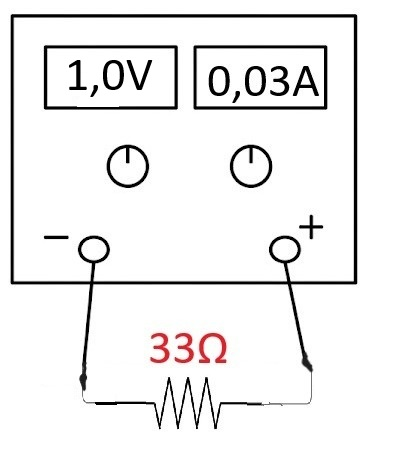
\includegraphics[width=0.6\textwidth]{img/Banco 2.jpg}\\	
  \caption{Banco de medición de la primer experiencia}
  \label{fig:figure1}
\end{figure}

\subsection{Análisis de los Resultados}

\begin{table}[h!]
  \begin{center}
    \label{tab:Tensión y corriente}  %etiqueta para referenciar la tabla
    \begin{tabular}{|c|c|c|c|c} % cantidad de columnas que va a tener representadas por las letras l, c, r, que indican el alineamiento (left, center, right). Una barra vertical "|" entre dos letras representa una linea dibujada entre las dos columnas
      \hline
      $V [V]$ & $\Delta V [V]$ & $I [A]$ & $\Delta I [A]$ \\ %los valores de cada columna, se separan con un "&". Al terminar con todas las columnas, se pasa a la siguiente línea con "\\".
      \hline
      1,00 & 0,10 & 0,03 & 0,01 \\ 
      \hline
      2,00 & 0,10 & 0,06 & 0,01 \\ 
      \hline
      3,00 & 0,10 & 0,09 & 0,01 \\ 
      \hline
      4,00 & 0,10 & 0,12 & 0,01 \\ 
      \hline
      5,00 & 0,10 & 0,16 & 0,01 \\ 
      \hline
      6,00 & 0,10 & 0,19 & 0,01 \\  
      \hline
      7,00 & 0,10 & 0,22 & 0,01 \\     
      \hline
      8,00 & 0,10 & 0,25 & 0,01 \\     
      \hline
      10,00 & 0,10 & 0,35 & 0,01 \\     
      \hline
      15,00 & 0,10 & 0,50 & 0,01\\     
      \hline
      \end{tabular}
    \caption{Mediciones de Tensión y Corriente}
  \end{center}
\end{table}

\begin{figure}[h!]
  \centering
  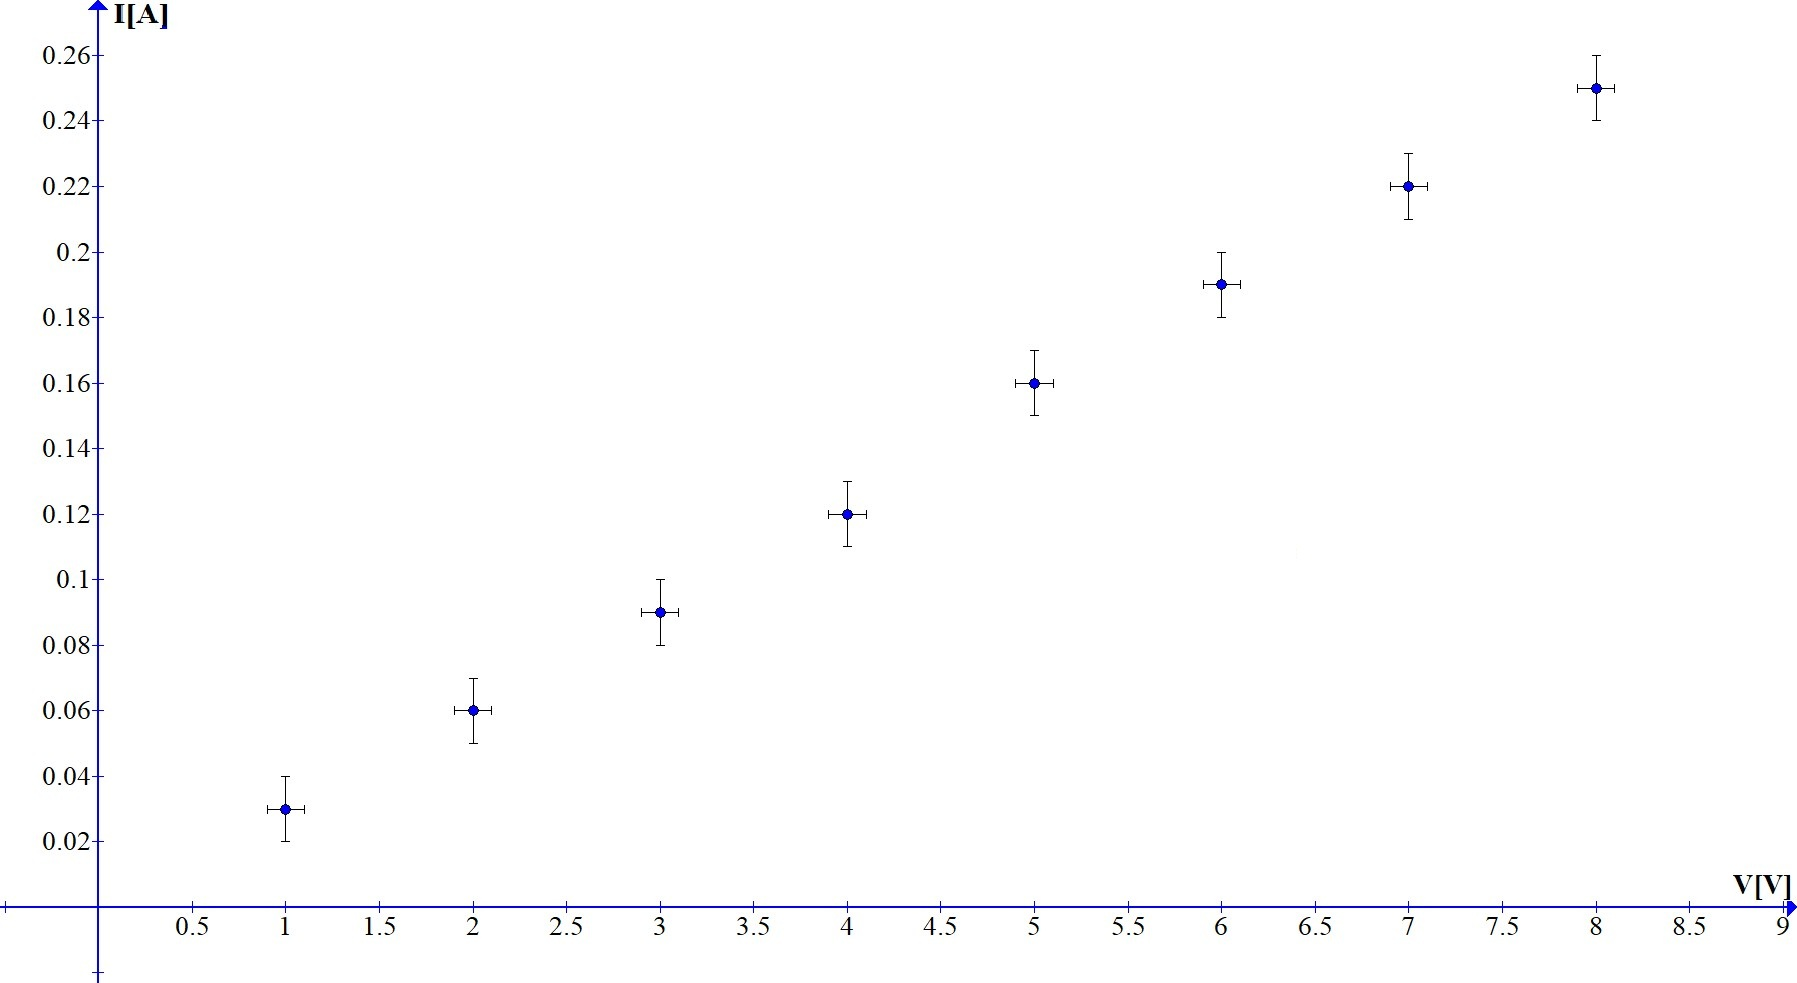
\includegraphics[width=0.9\textwidth]{img/I(T).jpg}\\	
  \caption{Gráfico de Corriente en función de la Tensión}
  \label{fig:figure1}
\end{figure}

Se observa en el gráfico de las mediciones (Figura 2) una tendencia lineal, es decir que existe una relación proporcionalmente directa entre la tensión y la corriente. Esto significa
que se puede calcular la constante que relaciona ambas variables, a la cual se denominará ``conductancia''. A la inversa de esta constante se le llama Resistencia, y se la
puede calcular a través de la Ley de Ohm: 

\begin{align}
    R = \frac{V}{I}
\end{align}

\begin{table}[h]
  \begin{center}
    \label{tab:Resistencias}  %etiqueta para referenciar la tabla
    \begin{tabular}{|c|c|c|c|c} % cantidad de columnas que va a tener representadas por las letras l, c, r, que indican el alineamiento (left, center, right). Una barra vertical "|" entre dos letras representa una linea dibujada entre las dos columnas
      \hline
      $V [V]$ & $I [A]$ & $R_1 [\Omega]$ & $\Delta R_1 [\Omega]$ \\ %los valores de cada columna, se separan con un "&". Al terminar con todas las columnas, se pasa a la siguiente línea con "\\".
      \hline
      1,00 & 0,03 & 33,33 & 11,60 \\ 
      \hline
      2,00 & 0,06 & 33,33 & 5,80 \\ 
      \hline
      3,00 & 0,09 & 33,33 & 3,87 \\ 
      \hline
      4,00 & 0,12 & 33,33 & 2,90 \\ 
      \hline
      5,00 & 0,16 & 31,25 & 2,05 \\ 
      \hline
      6,00 & 0,19 & 31,58 & 1,74 \\  
      \hline
      7,00 & 0,22 & 31,81 & 1,52 \\     
      \hline
      8,00 & 0,25 & 32,00 & 1,34 \\     
    \hline
      \end{tabular}
    \caption{Resistencia calculada}
  \end{center}
\end{table}

El valor de la incerteza fue calculado mediante el método de propagación de incertezas y los resultados anotados en el Cuadro 2. Si se observa su variación a lo largo de la 
tabla, se puede apreciar que a medida que se incrementan los valores de Tensión y Corriente, la incerteza de la Resistencia decrece. Esto indica que si hubiese que determinar la Resistencia a través de
una sola medición indirecta, sería conveniente usar una Tensión más alta para tener un valor más preciso de la Resistencia.

Por otro lado, se puede complementar el análisis de las incertezas con el intervalo de tolerancia dado por el fabricante. La resistencia tenía en la barra de tolerancia
el color dorado, que indica la resistencia puede variar $\pm {5} \% $ de su valor indicado. Un ${5} \% $ de $33 \Omega$ representa $1,65 \Omega $. 


\begin{figure}[h]
  \begin{center}
    \subfigure[Resitor de 33$\Omega$]{
        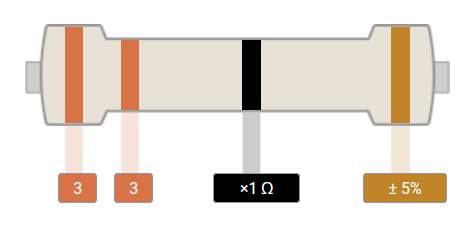
\includegraphics[width=0.4\textwidth]{img/Coloresd.png}
        \label{colores}}
    \subfigure[Código de colores]{
        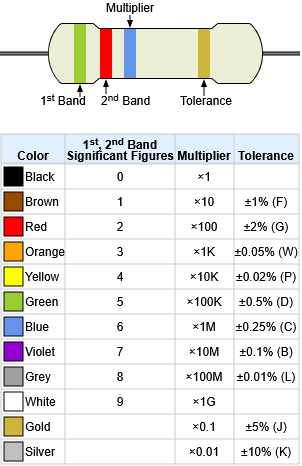
\includegraphics[width=0.3\textwidth]{img/Código.png}
        \label{código}}
    \caption{Código de colores y resistor}
    \label{fig:codigos}
  \end{center}
\end{figure}

A continuación se hace  comparación gráfica entre el intervalo de incertidumbre calculado de una de las mediciones indirectas, y el proporcionado por el fabricante:
\begin{figure}[h!]
  \centering
  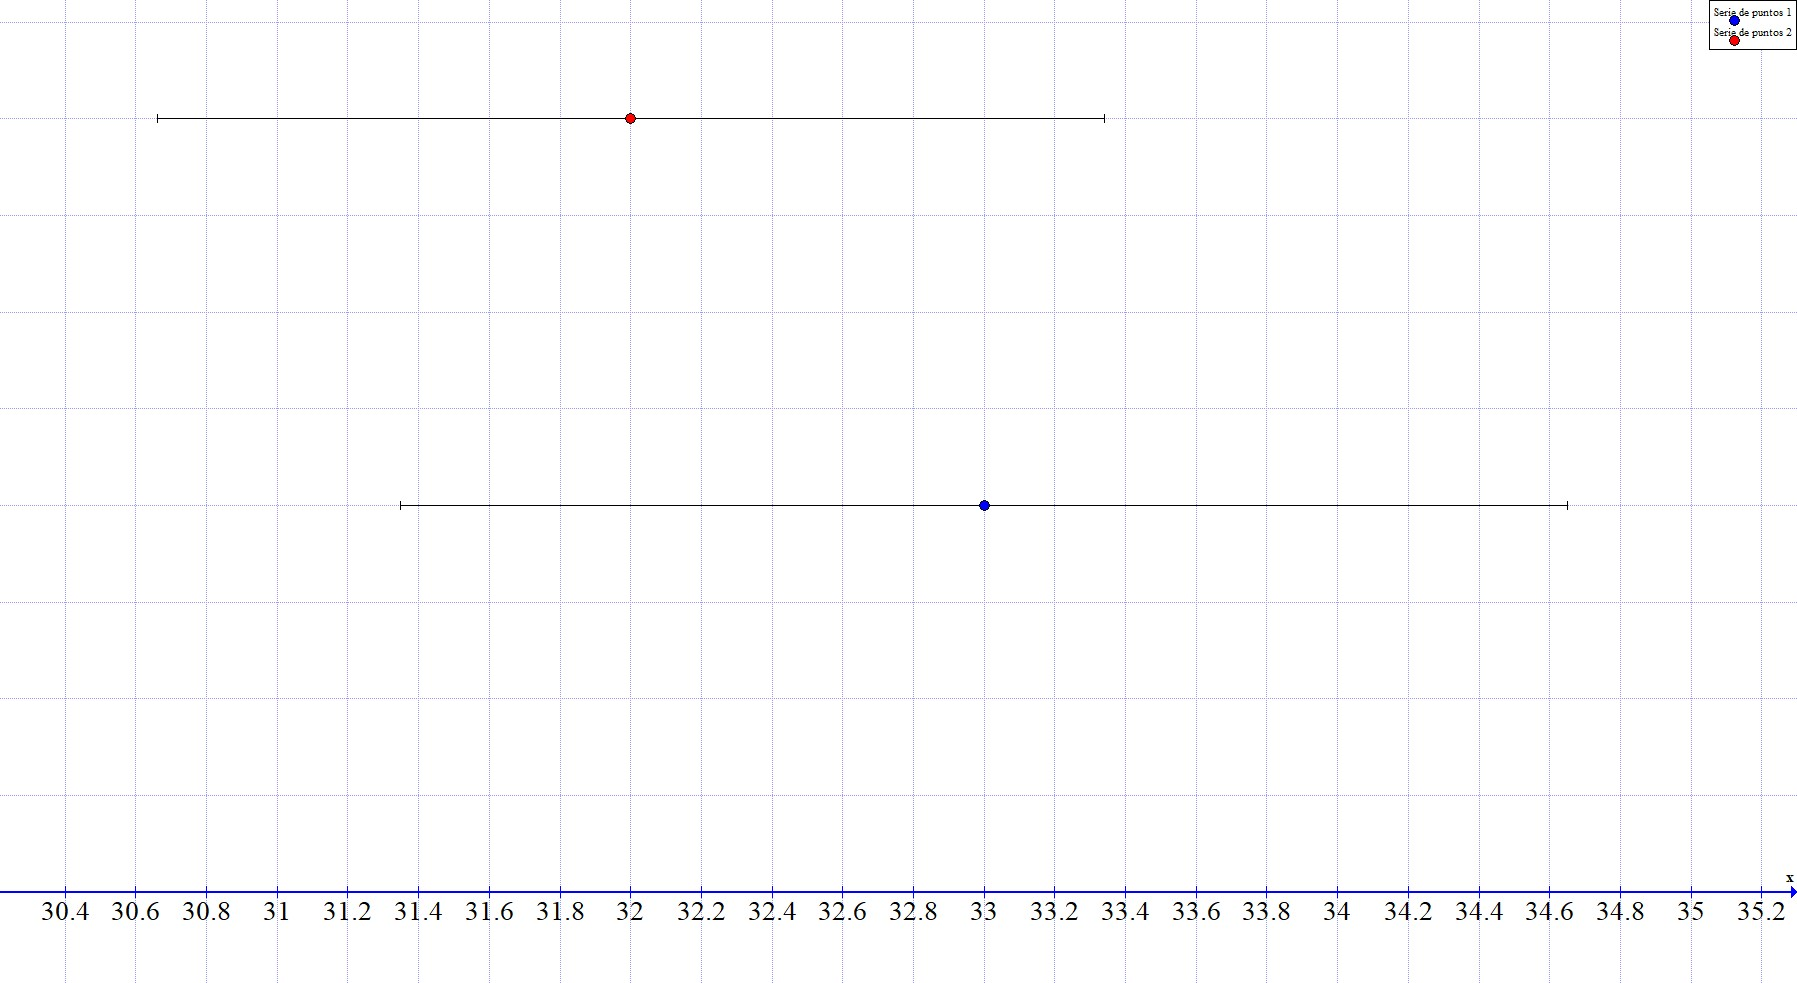
\includegraphics[width=1.1\textwidth]{img/incertezas.jpg}\\	
  \caption{Comparación gráfica de intervalos de incerteza del resistor}
  \label{fig:figure2}
\end{figure}

Un momento importante de la experiencia fue el aumentar la tensión lo suficiente para que se queme el resistor. 

Si la tensión supera el valor máximo que el resistor puede soportar, su temperatura se eleva significativamente, lo que puede provocar cambios en sus 
propiedades físicas (como variación de la resistencia) y eventualmente su deterioro o destrucción. Esto se manifiesta como un comportamiento no lineal en las mediciones que 
puede llegar a interrumpir el circuito.

Este fenómeno evidencia las limitaciones del modelo ideal de resistor, ya que en la práctica los componentes reales tienen restricciones térmicas que afectan su funcionamiento.
\section{Experiencia 2}

La segunda experiencia consistió en medir la tensión en diferentes puntos ($AB, BC, AC$) de dos circuitos diferentes, cada uno con dos resistencias conectadas en serie (Figura 4).

\begin{figure}[h]
  \begin{center}
    \subfigure[AB]{
        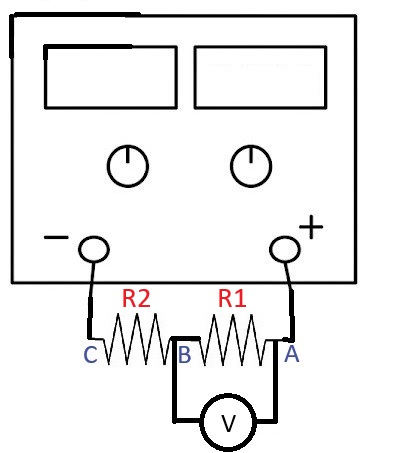
\includegraphics[width=0.33\textwidth]{img/Banco 1.jpg}
        \label{subfigAB}}
    \subfigure[BC]{
        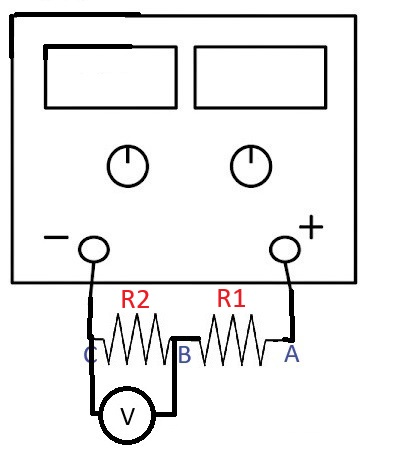
\includegraphics[width=0.33\textwidth]{img/Banco 12.jpg}
        \label{subfigBC}}
    \subfigure[AC]{
        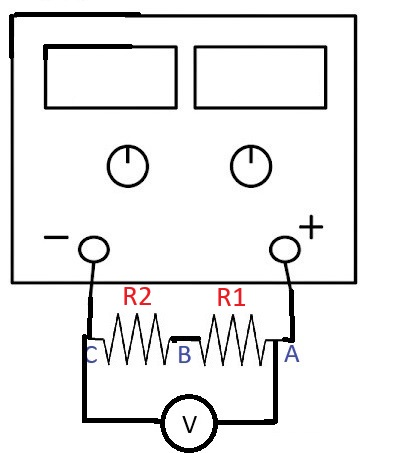
\includegraphics[width=0.33\textwidth]{img/Banco 13.jpg}
        \label{subfigAC}}
    \caption{Banco de medición en la segunda experiencia, con el multímetro en distintos puntos}
    \label{fig:image3}
  \end{center}
\end{figure}

\subsection{Análisis de los resultados}

\begin{table}[h]
  \begin{center}
    \label{tab:Tensión y corriente 2}  %etiqueta para referenciar la tabla
    \begin{tabular}{|c|c|c|c|c|c|c|c|c|} % cantidad de columnas que va a tener representadas por las letras l, c, r, que indican el alineamiento (left, center, right). Una barra vertical "|" entre dos letras representa una linea dibujada entre las dos columnas
      \hline
      & $R_{1} [\Omega]$ & $R_{2} [\Omega]$ & $I [A]$ & $\Delta I [A]$ & $V_{AB} [V]$ & $V_{AC} [V]$ & $V_{BC} [V]$ & $\Delta V [V]$ \\ %los valores de cada columna, se separan con un "&". Al terminar con todas las columnas, se pasa a la siguiente línea con "\\".
      \hline
      Circuito 1 & 33 & 56 & 0,02 & 0,01 & 3,10 & 5,00 & 1,80 & 0,10 \\  
    \hline
      Circuito 2 & $1000$ & $1000$ & 0,02 & 0,01 & 2,38 & 5,00 & 2,38 & 0,10 \\ 
          \hline
      \end{tabular}
    \caption{Mediciones de Tensión y Corriente}
  \end{center}
\end{table}

Teniendo en cuenta la ley de Ohm:
\begin{align}
    V_{f} & = I \cdot (R_{1}+R_{2}) \\
    I & = \frac{V_{f}}{(R_{1}+R_{2})}
\end{align}
Entonces las caídas de tensión en el primer caso son:

\begin{align}
    V_{AB} = V_{R1} & = I \cdot R_{1} = \frac{V_{f} \cdot R_{1}}{(R_{1}+R_{2})} = \frac{5V \cdot 33\Omega}{{33}{\Omega}+{56}{\Omega}}=1,85V\\
    V_{BC} = V_{R2} & = I \cdot R_{2} = \frac{V_{f} \cdot R_{2}}{(R_{1}+R_{2})} = \frac{5V \cdot 56\Omega}{{33}{\Omega}+{56}{\Omega}}=3,15V
\end{align}

Comparando con los valores de la tabla, se observa que la diferencia entre los valores experimentales y teóricos es bastante baja, de solamente 0,05V (dentro
del margen de incertidumbre). Igualmente se puede explicar que haya caídas de tensión ``ocultas'' fuera de R1 y R2 por la resistencia que opone el instrumento de medición, 
despreciable en este caso. Si se suma $V_{R1}+V_{R2}$ experimentales, el resultado es 4,90V, que se encuentra en el margen de incertidumbre, por lo que se puede afirmar
que se verifica la ley de Kirchhoff, dentro del error experimental. 

En el segundo circuito, se obtienen resultados ideales un poco más alejados del experimento: 
\begin{align}
    V_{AB} = V_{R1} & = I \cdot R_{1} = \frac{V_{f} \cdot R_{1}}{(R_{1}+R_{2})} = \frac{5V \cdot 1000\Omega}{{1000}{\Omega}+{1000}{\Omega}}=2,5V\\
    V_{BC} = V_{R2} & = I \cdot R_{2} = \frac{V_{f} \cdot R_{2}}{(R_{1}+R_{2})} = \frac{5V \cdot 1000\Omega}{{1000}{\Omega}+{1000}{\Omega}}=2,5V
\end{align}

Si se suman de los valores experimentales $V_{R1}+V_{R2}$, el resultado es 4,76V, que tiene una diferencia de 0,26V con respecto al valor ideal. Kirchhoff debería cumplirse, 
pero ahora el desvío es más grande que antes, y esto evidencia que el modelo ideal del circuito es incompleto, porque ignora las resistencias ``ocultas'' que se mencionaron antes.
En este caso, el valor de resistencia que oponen los cables, la fuente y el propio multímetro modifican el circuito. El instrumento funciona en paralelo con 
los resistores, que estando en serie producen una resistencia equivalente muy alta pero el multímetro reduce la resistencia total equivalente (está en paralelo) y cae la tensión.

\subsection{Generalización a N resistores en serie}
La segunda ley de Kirchoff expresa lo siguiente:
\begin{align}
  \sum_{i=1}^{n} V_{k} = 0
\end{align}
Esto significa que la suma de las caídas de tensiones es igual a la tensión de la fuente, entonces:
\begin{align}
  I \cdot \sum_{i=1}^{n} R_{k} = V_{f}\\
  I = \frac{V_{f}}{\sum_{i=1}^{n} R_{k} }
\end{align}
La caída de tensión en cada resistor se calcula así:
\begin{align}
  V_{Ri}=I\cdot R_{i}
\end{align}
Y si se reemplaza:
\begin{align}
  V_{Ri}= \frac{V_{f} \cdot R_{i}}{\sum_{i=1}^{n} R_{k} }
\end{align}

De esta forma se obtiene la expresión de la caída de tensión en función de la resistencia e independiente de la corriente.

\subsection{Simulación del circuito}
\begin{figure}[h]
  \begin{center}
    \subfigure[Circuito]{
        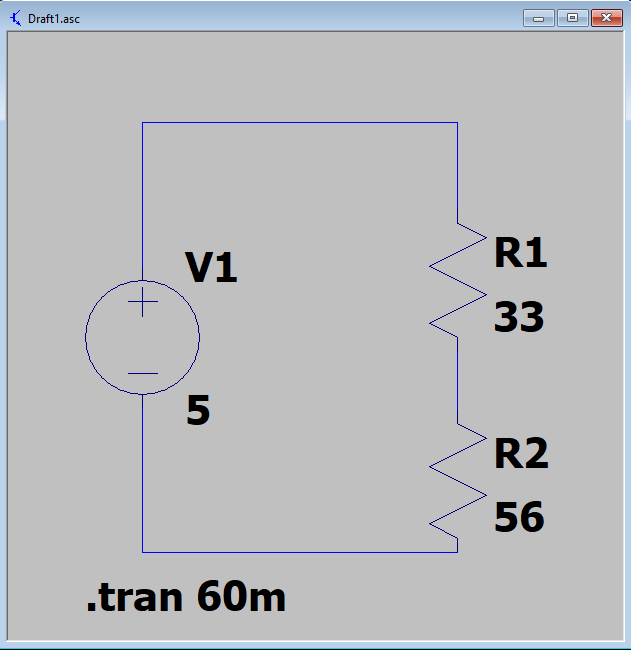
\includegraphics[width=0.3\textwidth]{img/litspice.png}
        \label{litspice}}
    \subfigure[Plot (Azul punteado: R1, Verde: R2)]{
        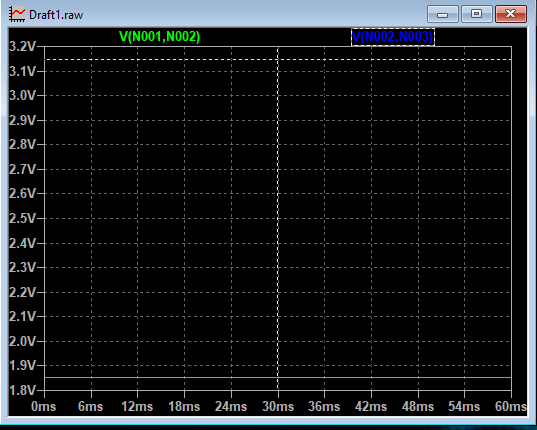
\includegraphics[width=0.6\textwidth]{img/litspice plot.png}
        \label{plot}}
    \caption{Simulación en el programa Litspice}
    \label{fig:image22}
  \end{center}
\end{figure}
Utilizando el programa Litspice se diseñó el circuito de la segunda experiencia para que el programa simule corriente y tensión sobre este diseño )Figura 5). 
Los resultados de la simulación fueron $V1=1.8539326V$ y $V2=3.1460673V$, lo cual indica que el programa por ``default'' hace una medición que toma todos los componentes como ideales 
(la suma de ambas tensiones es igual a la de la fuente). Luego se comprobó qué sucede si se le pide a una IA del tipo LLM, en este caso ChatGPT, que confeccione el circuito para simular 
en un archivo ``.asc'' (Figura 6).
\begin{figure}[h!]
  \begin{center}
    \subfigure[Circuito]{
        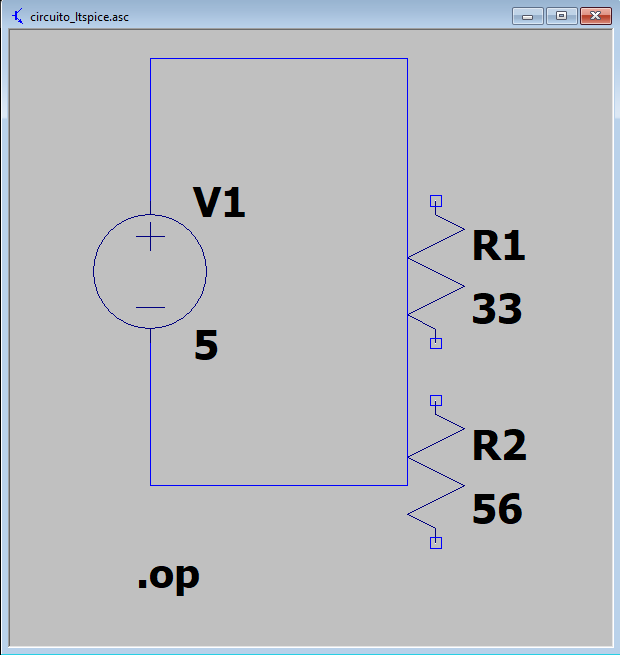
\includegraphics[width=0.3\textwidth]{img/litspc.png}
        \label{litspicegpt}}
    \subfigure[Mensaje de ``Nothing to solve.'']{
        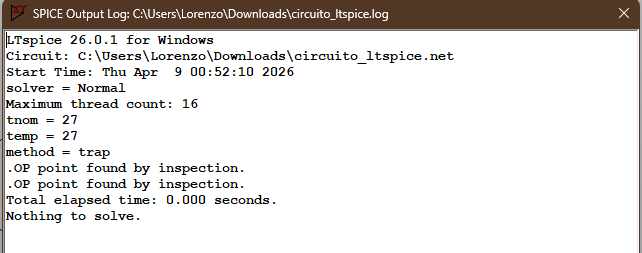
\includegraphics[width=0.6\textwidth]{img/litspacegpt.png}
        \label{plotGPT}}
    \caption{Simulación en el programa Litspice con un archivo hecho con IA}
    \label{fig:litspacegpty}
  \end{center}
\end{figure}

Es claro que ChatGPT no tuvo la capacidad de realizar bien el esquema del circuito: se observa que en su esquema  ambas resistencias están desconectadas y por eso el programa no tiene ``nada
que resolver''.

\section{Conclusiones}
En la primera experiencia se estudió la relación entre la tensión y la corriente en un resistor, verificándose un comportamiento lineal entre ambas magnitudes. 
Esto permitió confirmar la validez de la Ley de Ohm dentro del rango de mediciones realizadas. A partir de los datos experimentales se determinó el valor de la resistencia, 
obteniéndose resultados compatibles entre sí y coherentes con la tolerancia indicada por el fabricante.

Además, se observó que la incertidumbre en la determinación de la resistencia disminuye al aumentar los valores de tensión y corriente medidos, lo cual indica 
que es conveniente trabajar en ese rango para obtener mayor precisión. El resistor cumple la función de oponerse al paso de la corriente eléctrica, y ante corrientes elevadas
puede sobrecalentarse y eventualmente dañarse.

En la segunda experiencia se analizaron circuitos con resistores en serie, verificándose la ley de Kirchhoff de tensiones dentro del margen de error experimental. 
Se observó que las discrepancias entre los valores teóricos y experimentales aumentan en circuitos con resistencias más altas, 
lo cual puede atribuirse a la influencia de resistencias no ideales presentes en los instrumentos de medición, cables y fuente.

Finalmente, la simulación permitió comparar un modelo ideal con el comportamiento real del circuito, evidenciando que los modelos teóricos simplifican 
el sistema al no considerar ciertos efectos presentes en la práctica. En conjunto, los resultados obtenidos permiten concluir que los modelos estudiados 
describen adecuadamente el comportamiento eléctrico en condiciones controladas, aunque presentan limitaciones frente a situaciones reales.

\end{document}
